\section{Classification and Prediction}
Artificial neurons can perform two different actions: classification and prediction. Originally, the idea of the
perceptron was to be a binary classifier, but it can actually do more. In this chapter, we will see how
to adapt the neuron to predict values, but first lets see what does exactly means classification and prediction.

\begin{itemize}
\item \textbf{Classification:} is the process of assigning a label to an input data point.
  For example, a classification model could be used to determine whether an email is spam or not spam, or
  whether a patient has a certain disease or not. We have already explored this concept in the previous chapter,
  where we provided examples using logic gates and a simple image classifier.
  
\item \textbf{Prediction:} is the process of estimating the value of a target variable based on a set of
  input variables. For example, a prediction model could be used to estimate the price of a house, or the
  likelihood of a customer clicking on an ad.
\end{itemize}

The perceptron can be utilized as a prediction model through a technique called linear regression.
Let's first delve into how linear regression works.

\subsection{How linear regression works?}
Linear regression is a statistical method that finds a linear relationship between the independent variables
and the dependent variable. This means that the relationship between the independent variables and
the dependent variable can be modeled by a straight line.\\
The independent variables are the variables that we believe influence the dependent variable. In the case
of predicting the price of a house, some independent variables might be the size of the house, the number of
bedrooms, the location of the house, and the age of the house.\\
The dependent variable is the variable that we are trying to predict. In the case of predicting the
price of a house, the dependent variable is the price of the house.\\
Linear regression can be geometrically represented as a line that best fits the data points in a dataset.
The independent variables are represented by the horizontal axis $\vec{x}$,
and the dependent variable is represented
by the vertical axis $y$. The line that best fits the data points is the one that minimizes the distance between
the line and the data points.


\begin{figure}[H]
  \centering
  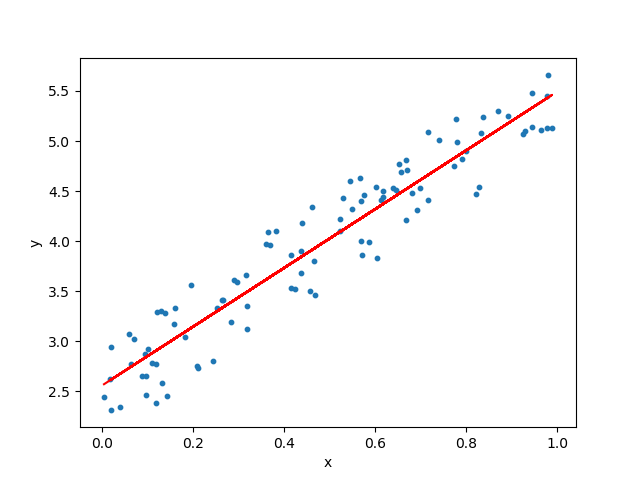
\includegraphics[scale = 0.38]{linear_regression.png}
  \caption{Linear regression.}
\end{figure}

The perceptron algorithm is a binary classifier that creates a linear decision boundary to separate data into two
categories. This is similar to linear regression, which also uses a linear boundary. However, linear regression
predicts continuous values, while the perceptron algorithm classifies data into distinct categories.
The perceptron learns from labeled examples to find the optimal boundary that separates the data effectively.

\begin{figure}[H]
  \centering
  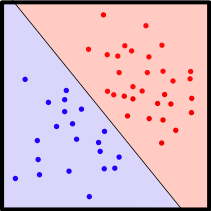
\includegraphics[scale = 0.8]{linearly.png}
  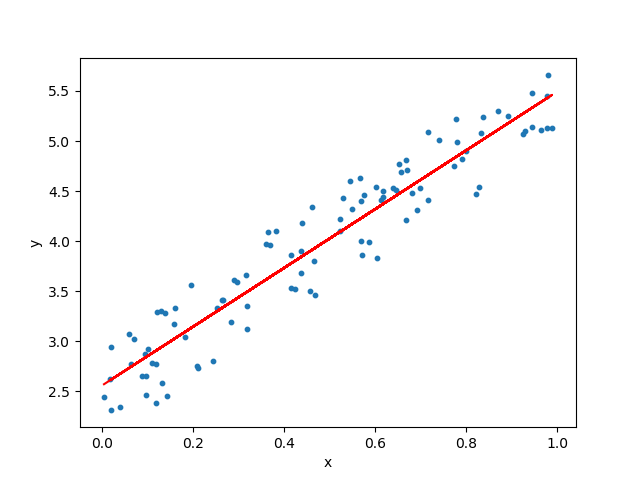
\includegraphics[scale = 0.4]{linear_regression.png}
  \caption{The linear separability and the linear regression}
\end{figure}

\section{Coding the prediction perceptron}
\subsection{Modifying the perceptron algorithm}
We have observed that the perceptron algorithm involves a dot product operation between the input components and
corresponding weights, given by $\sum_{i = 0}^n(x_i \cdot w_i) = \vec{x} \cdot \vec{w}$. Here,
$\vec{x} = \{1, x_1, x_2, \ldots, x_n\}$ represents the input vector, $\vec{w} = \{b, w_1, w_2, \ldots, w_n\}$
represents the weight vector, where $b = w_0$ and $1 = x_0$. This dot product is then passed through an
activation function.

We can express the output as $y = \text{activation}(\vec{x} \cdot \vec{w})$. The activation function maps the
result to a domain of $\{x_0, x_1\}$, depending on the chosen activation function.

To predict continuous values, we don't need an activation function because our outputs are not restricted to a
finite group of values like $\{x_0, x_1\}$. Instead, we require the entire domain, which can be represented
by $\mathbb{R}$ or $\mathbb{Z}$ depending on the type of value we are trying to predict. In some cases, we may
need to make convenient modifications to map values from $\mathbb{R}$ to another infinite group of values.

The algorithm can be simply understood as a dot product of vectors.
\[
f(\vec{x}) = \vec{w} \cdot \vec{x} \quad | \quad \vec{x} = \{1, x_1, \cdots, x_n\},
\vec{w} = \{b, w_1, \cdots, w_n \}
\]

\subsection{From linear regression algorithm to code}
First, declare your weights. Remember that the weights already include the bias or threshold, represented
as $\vec{w} = \{b, w_1, \cdots, w_n\}$. Therefore, you need to insert a value of 1 for each input data that you
want to provide to the perceptron, represented as $\vec{x} = \{1, x_1, \cdots, x_n\}$.
\begin{verbatim}
weights = [4.1, 0.0, 2.0, 1.0, 2.8] // 4.1 = b = w_0
input = [1.0, 23.0, 42.0, 12.0, 21.0] // 1.0 = x_0
\end{verbatim}
Next, you only need to sum and multiply each element and return the sum as it will represent the predicted value.
\begin{verbatim}
sum = 0.0
for (i = 0, i < input.length, i++)
    sum += input[i] * weights[i]
return sum
\end{verbatim}
The predicted value is computed through a dot product operation between the input vector and the weight vector.
This enables us to estimate continuous values and make predictions. To train this modified perceptron, we need
to adjust the weights. The training process involves iteratively updating the weights based on prediction
errors. 
\subsection{A simple training algorithm for predicting values}
To train a linear regression neuron, we can adjust the weights based on prediction errors.
In addition to the perceptron training algorithm, there are various approaches available for this purpose,
including popular ones like gradient descent and backpropagation, which will be covered extensively in the
subsequent chapters. These algorithms provide powerful techniques for refining the neuron's parameters and
optimizing its predictive performance. However, for our current focus on linear regression neurons, we will
utilize a modified version of the perceptron training algorithm. This modified approach allows us to
iteratively update the weights by considering the discrepancies $\varepsilon$ between predicted values and
the true target
values. By systematically adjusting the weights, we aim to minimize these prediction errors and improve the
accuracy of our linear regression neuron.
Actually, the learning algorithm we are going to use for this regression will be very similar to
the perceptron learning algorithm because
it shares almost the same characteristics. The main difference is that, for each iteration, it will update
the weights. Remember, our goal is to minimize the discrepancy, $\varepsilon$, as much as possible.
In simpler terms, the linear regression neuron learning process can be summarized in these three steps:
\begin{enumerate}
\item The training function makes predictions based on the activation function, which can be represented
  as $f(\vec{x}_t) = \vec{x}_t \cdot \vec{w}_k$, where $t$ denotes the current iteration through the training
  data, and $k$ represents the current state of the weights.

\item The perceptron for each $t$ iteration will adjusts its weights. Again there are different
  ways to perform this
  adjustment, but one common approach that we can use is to utilize useful information such as the input
  vector $\vec{x}$,
  the discrepancy, $\varepsilon$, which can be computed $\varepsilon = y_t - f(\vec{x}_t)$  where $y_t$ is the
  desired prediction,
  and a learning rate $\gamma$ (where $\gamma$ is a small value, $\gamma < 1$).
  The weight adjustment can be expressed as $\vec{w}_{k+1} = \vec{w}_k + \gamma \varepsilon \vec{x}_t$.

\item After many predictions and adjustments, the weights will converge to the desired weights denoted as
  $\vec{\theta}^*$, which can be represented as
  $k \rightarrow \infty \quad \implies \quad \vec{w}_k \rightarrow \vec{\theta}^*
  ,\quad \varepsilon \rightarrow 0$.
\end{enumerate}

By following these steps, the neuron learns and adapts its weights until it achieves accurate predictions.

\subsubsection{The Math Intuition of Linear Regression}
The goal of linear regression is to estimate the coefficients that best fit the observed data. In matrix notation
, the model can be represented as $y = X\beta + \varepsilon$, where $y$ is the vector of dependent variable
values,
$X$ is the matrix of independent variable values, $\beta$ is the vector of coefficients, and $\varepsilon$ is
the error term. The error term captures the discrepancy between the actual values of the dependent variable and
the values predicted by the linear regression model. By minimizing these discrepancies, the model aims to
find the
coefficients that provide the best overall fit to the data.
\begin{figure}[H]
  \centering
  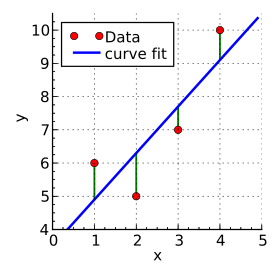
\includegraphics[scale = 1]{linear_regression2.png}
  \caption{In linear regression, the observations (red) are assumed to be the result of random deviations
    (green) from an underlying relationship (blue) between a dependent variable ($y$) and an independent
    variable ($x$).}
\end{figure}

\subsection{From Learning Algorithm to Code}
The learning algorithm we are going to use is similar to the perceptron learning algorithm.
First, you need to define the learning rate $\gamma$ and the number of iterations $t$ for training:
\begin{verbatim}
learning_rate = 0.01
num_epochs = 100
\end{verbatim}
The implementation of this training algorithm involves nested for loops, similar to the
perceptron learning algorithm. The `inputs` array should be a bidimensional array.

\begin{verbatim}
for (i = 0; i < num_epochs; i++)
    for (j = 0; j < inputs.length; j++)
        sum = 0.0;
        for (k = 0; k < weights.length; k++)
            sum += inputs[j][k] * weights[i];
\end{verbatim}
Within the innermost loop iterating over the inputs, you will update the weights:
\begin{verbatim}
error = output[j] - sum;
for (k = 0; k < weights.length; k++)
    weights[k] += learning_rate * error * inputs[j][k];
\end{verbatim}
This code segment outlines the general structure of the learning algorithm.

\section{The math behind of the learning algorithm}
When using the linear regression neuron for prediction instead of classification, there will always
be a discrepancy, denoted as $\varepsilon$. This discrepancy can be calculated as follows:
\[
\varepsilon_t = y_t - \vec{w}_k \cdot \vec{x}_t
\]
Ultimately, our goal is to find a desired vector $\vec{\theta}^*$ that minimizes the
discrepancy $\varepsilon$ for all possible inputs. Mathematically, this can be expressed as:
\[
\exists \vec{\theta}^* \in \mathbb{R}^{d} \quad|\quad \forall \text{min}\{\varepsilon_t\}
\]
where
\[
\varepsilon_t = y_t - \vec{\theta}^* \cdot \vec{x}_t\quad|\quad \forall(\vec{x}_t, y_t) \in \mathbb{D}
\]
Here, $(\vec{x}_t, y_t) \in \mathbb{D}$ represents the entire dataset.

The fundamental idea is to utilize $\varepsilon_t$ as a direction and proportion to iteratively
adjust the weights, resulting in an update equation like this:
\[
\vec{w}_{k + 1} = \vec{w}_{k} + \varepsilon_t \cdot \vec{x}_t
\]
Intuitively, consider the following expressions:
\[
\varepsilon_t < 0 \Longleftrightarrow y_t < \vec{w}_k \cdot \vec{x}_t
\Longleftrightarrow \vec{w}_{k + 1} < \vec{w}_k
\]

\[
\varepsilon_t > 0 \Longleftrightarrow y_t > \vec{w}_k \cdot \vec{x}_t
\Longleftrightarrow \vec{w}_{k + 1} > \vec{w}_k
\]

In the algorithm, we aim to make the weight adjustments less aggressive.
To understand why we adjust the weights in this manner, consider the following illustration.

\begin{center}
\begin{tikzpicture}[scale=1.5]
  \draw[thick,->] (2,0) -- (0,1) node[anchor=south west]{$\vec{w}_k$};
  \draw[thick,->] (2,0) -- (5,0) node[anchor=south west]{$\vec{\theta}^*$};
\end{tikzpicture}
\end{center}

Here, $\vec{\theta}^*$ represents the desired vector configuration, while $\vec{w}_k$ corresponds to the
current iteration's weights. Although we do not know the exact position of $\vec{\theta}^*$, we
can approximate $\vec{w}_k$ to $\vec{\theta}^*$ by adding vectors. Consequently, we can introduce
the vector $\varepsilon_t \cdot \vec{x}_t$ to the illustration.

\begin{center}
\begin{tikzpicture}[scale=1.5]
  \draw[thick,->] (2,0) -- (0,1) node[anchor=south west]{$\vec{w}_k$};
  \draw[thick,->] (2,0) -- (5,0) node[anchor=south west]{$\vec{\theta}^*$};
  \draw[thick,->] (2,0) -- (5,-1) node[anchor=south west]{$\varepsilon_t\vec{x}_t$};
\end{tikzpicture}

\begin{tikzpicture}[scale=1.5]
  \draw[thick,->] (2,0) -- (0,1) node[anchor=south west]{$\vec{w}_k$};
  \draw[thick,->] (2,0) -- (5,0) node[anchor=south west]{$\vec{\theta}^*$};
  \draw[thick,->] (2,0) -- (5,-1) node[anchor=south west]{$\varepsilon_t\vec{x}_t$};

  \draw let \p1 = (-2,1), \p2 = (5,-1.78), \n1 = {atan2(\y1,\x1)}, \n2 = {atan2(\y2,\x2)} in (2,0) + (\n1:0.8) arc (\n1:\n2:0.8) node[midway, above right] {$\theta$};
\end{tikzpicture}
\end{center}

Recall that adding two vectors together results in their rotation. Hence,
the computation of $\vec{w}_{k + 1}$ must bring it closer to $\vec{\theta}^*$.


So think in the addition of vector as way to rotate a vector, look if I sum $\vec{w}_k + \varepsilon_t\vec{x}_t$
I get the next iteration the $k + 1$ iteration which results on this new vector $\vec{w}_{k + 1}$.
\begin{center}
\begin{tikzpicture}[scale=1.5]
  \draw[thick,->] (2,0) -- (0,1) node[anchor=south west]{$\vec{w}_k$};
  \draw[thick,->] (2,0) -- (5,0) node[anchor=south west]{$\vec{\theta}^*$};
  \draw[thick,->] (2,0) -- (5,-1) node[anchor=south west]{$\varepsilon_t\vec{x}_t$};
  \draw[thick,->] (2,0) -- (3,0.5) node[anchor=south west]{$\vec{w}_{k + 1} = \vec{w}_k + \varepsilon_t\vec{x}_t$};
  \draw[dashed] (0,1) -- (3,0.5);
  
  \draw let \p1 = (2,1), \p2 = (5,-1.78), \n1 = {atan2(\y1,\x1)}, \n2 = {atan2(\y2,\x2)} in (2,0) + (\n1:0.8) arc (\n1:\n2:0.8) node[midway, above right] {$\theta$};
\end{tikzpicture}
\end{center}

Finally, through the \hyperref[sec:perceptron-convergence-proof]{convergence proof of the perceptron},
we can be confident that
$\vec{w}_k$ will converge to the desired vector of weights, $\vec{\theta}^*$.

\section{Examples}
By comprehending the underlying linear regression algorithm
and its convergence properties, we have uncovered the key principles
behind its functionality. The availability of practical code examples further enhances our understanding and
allows for easy implementation. You can find a collection of these illustrative examples in the provided
GitHub repository at the following link:
\href{https://github.com/alecksandr26/fortran-ml/tree/main/examples}{examples}.
\subsection{Linear regression neuron module in fortran}
I have developed a simple linear regression neuron  module in Fortran, which includes the weights.
The module encompasses subroutines for training and testing the
neuron. To delve deeper into the implementation details, you can access the source code
\href{https://github.com/alecksandr26/fortran-ml/tree/main/src/mod_linear_regression.f90}{here}.

\begin{lstlisting}
module mod_linear_regression
  use iso_fortran_env, only : real32, int32
  use assertf
  implicit none

  private
  public lr_init, lr_free, linear_regression, lr_train, lr_test

  type linear_regression
     integer(int32) :: n
     real(real32), pointer :: w(:)
  end type linear_regression
  
contains
  
  subroutine lr_init(lr, w)
    real(real32), intent(in) :: w(:)
    type(linear_regression), intent(out) :: lr

    ! Fetch the size from the array
    lr%n = size(w)

    allocate(lr%w(lr%n))
    
    ! Copy the initial weights 
    lr%w(:) = w(:)
  end subroutine lr_init

  subroutine lr_free(lr)
    type(linear_regression), intent(in out) :: lr
    deallocate(lr%w)
    lr%n = 0
  end subroutine lr_free

  subroutine lr_train(lr, inputs, outputs, lrate, nepochs)
    type(linear_regression), intent(in out) :: lr
    real(real32), intent(in) :: inputs(:, :), outputs(:)
    real(real32), intent(in) :: lrate
    integer(int32), intent(in) :: nepochs

    integer(int32) :: n
    real(real32), allocatable :: results(:)
    integer(int32) :: i, j, k
    
    n = size(outputs)
    allocate(results(n))

    do concurrent(i = 1 : nepochs)
       do concurrent(j = 1 : n)
          ! Vector multiplication w * x
          results(j) = 0
          do concurrent(k = 1 : lr%n)
             results(j) = results(j) + lr%w(k) * inputs(k, j)
          end do

          ! Update the weights
          do concurrent(k = 1 : lr%n)
             lr%w(k) = lr%w(k) + lrate * (outputs(j) - results(j)) * inputs(k, j)
          end do
       end do
    end do
    deallocate(results)
  end subroutine lr_train

  subroutine lr_test(lr, input, output)
    type(linear_regression), intent(in out) :: lr
    real(real32), intent(in) :: input(:)
    real(real32), intent(out) :: output
    integer(int32) k

    do concurrent(k = 1 : lr%n)
       output = output + lr%w(k) * input(k)
    end do
  end subroutine lr_test
  
end module mod_linear_regression
\end{lstlisting}

\subsection{Predicting sales}
This scenario involves a fundamental prediction task: estimating the potential earnings of a product or
service after a specific number of days of sales, such as forecasting the revenue generated after 11 days.
In such cases, linear regression emerges as the ideal approach for making accurate predictions. With its
ability to capture linear relationships between variables, linear regression proves to be a suitable candidate
for predicting future outcomes in this context.\\

In this simple program written in Fortran, I utilized the previously demonstrated Fortran module for performing
linear regression. In basic terms, the program prints the data being used and proceeds to predict the output
for each input, displaying the results.
\begin{lstlisting}
program example
  use iso_fortran_env, only : real32, int32
  use mod_linear_regression
  use assertf
  implicit none

  type(linear_regression) :: lr
  real(real32) :: inputs(2, 7) = reshape([1, 4, 1, 5, 1, 6, 1, 7, 1, 8, 1, 9, 1, 10], [2, 7])
  ! inputs = [[1, 4], [1, 5], [1, 6], [1, 7], [1, 8], [1, 9], [1, 10]]
  real(real32) :: outputs(7) = [50, 70, 72, 73, 90, 95, 105]
  real(real32) :: output = 0.0
  integer(int32) :: i = 0

  write(*, '(A)', advance='no') "inputs: "
  do i = 1, size(inputs, 2)
     write(*, '(F0.1, A)', advance='no') inputs(2, i), ' '
  end do
  write(*,*)

  write(*, '(A)', advance='no') "outputs: "
  do i = 1, size(outputs)
     write(*, '(F0.1, A)', advance='no') outputs(i), ' '
  end do
  write(*,*)
  

  call lr_init(lr, [0.0, 0.0])
  call lr_train(lr, inputs, outputs, 0.0001, 4000000)

  write(*, '(A)', advance='no') "results: "
  do i = 1, size(inputs, 2)
     call lr_test(lr, inputs(:, i), output)
     write(*, '(F0.1, A)', advance='no') output, ' '
     output = 0.0
  end do
  write(*,*)

  write(*, '(A)', advance='no') "weights: "
  write(*, '(F0.1, A, F0.1)', advance='no') lr%w(1), ' ', lr%w(2)
  write(*,*)
  
  call lr_free(lr)
end program example 
\end{lstlisting}
The module of linear regression works as the \hyperref[sec:perceptron-module-fortran]{perceptron module}.

\subsubsection{Output}
\begin{verbatim}
inputs: 4.0 5.0 6.0 7.0 8.0 9.0 10.0 
outputs: 50.0 70.0 72.0 73.0 90.0 95.0 105.0 
results: 54.3 62.6 70.9 79.3 87.6 95.9 104.3 
weights: 21.0 8.3  
\end{verbatim}
\subsubsection{Picture of the results}
This is the result of the line. As you can see, the neuron learns after iterating with a lot of epochs.

\begin{figure}[H]
  \centering
  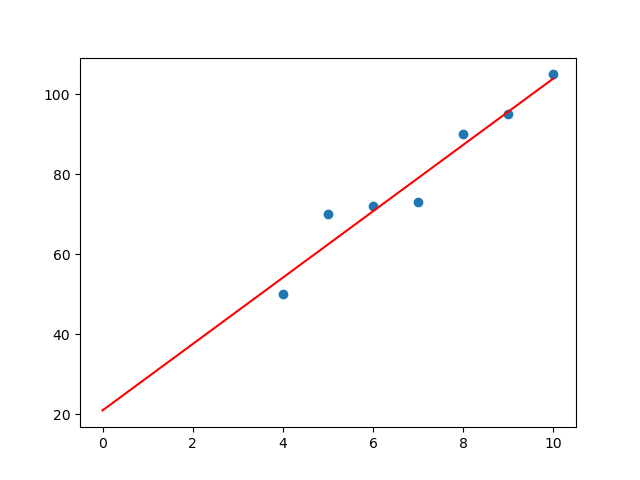
\includegraphics[scale = 0.9]{sales_prediction.png}
  \caption{Results of the linear regression neuron.}
\end{figure}

\subsection{Stock price prediction}
In the previous chapter, we delved into a simple example to grasp the fundamentals. Now, let's take on a more
realistic scenario. To accomplish this, we'll work with the 'TESLA.csv' file, which can be accessed through the
provided link. This file contains a comprehensive dataset encompassing various aspects of Tesla's stock prices,
including significant labels such as Date, Open, High, Low, Close, Adj Close, and Volume.

Our objective is to predict the closing price of Tesla's stock by considering multiple factors. These factors
include the date, represented as a numerical value, along with the opening price, high price, low price, and
volume of stocks exchanged.

Let's take a closer look at the initial lines of the .csv file:
\begin{verbatim}
Date,Open,High,Low,Close,Adj Close,Volume
2020-01-02,84.900002,86.139999,84.342003,86.052002,86.052002,47660500
2020-01-03,88.099998,90.800003,87.384003,88.601997,88.601997,88892500
2020-01-06,88.094002,90.311996,88.000000,90.307999,90.307999,50665000
2020-01-07,92.279999,94.325996,90.671997,93.811996,93.811996,89410500
2020-01-08,94.739998,99.697998,93.646004,98.428001,98.428001,155721500
2020-01-09,99.419998,99.760002,94.573997,96.267998,96.267998,142202000
2020-01-10,96.358002,96.987999,94.739998,95.629997,95.629997,64797500
2020-01-13,98.699997,105.125999,98.400002,104.972000,104.972000,132588000
2020-01-14,108.851997,109.482002,104.980003,107.584000,107.584000,144981000
\end{verbatim}
Training this type of neuron posed challenges due to the complexity of achieving linear separability.
The initial hurdle I encountered was determining the appropriate learning rate. Since these models learn by
iteratively adjusting weights based on nearly random differences, selecting an unsuitable learning rate could
prevent convergence. Consequently, a second issue arose: striking a balance between convergence and training
time. To ensure convergence, I had to opt for an extremely small learning rate, which in turn necessitated a
substantial number of epochs. As a result, I spent countless hours training the model without achieving
satisfactory outcomes. To illustrate, consider the accompanying images: the red dots represent predicted
values, while the blue dots represent actual values.

\begin{figure}[H]
  \centering
  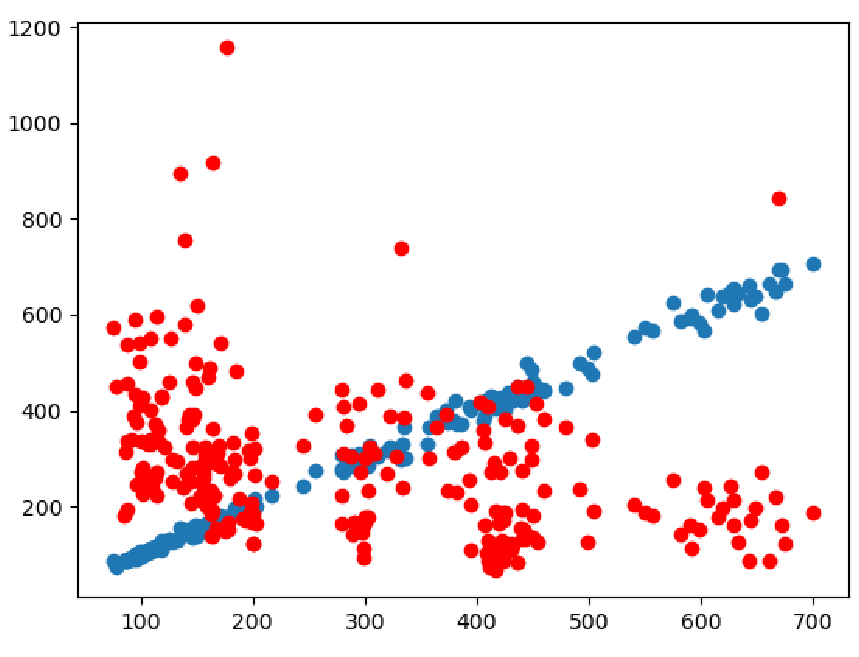
\includegraphics[scale = 0.4]{stock_prediction2.png}
  \caption{Results of the linear regression neuron predicting the stock.}
\end{figure}

As you can observe from the results, the predictions obtained were not satisfactory. In an attempt to improve
the model's performance, a decision was made to remove one of the independent variables, namely the Volume.
This reduction resulted in a model with four dimensions, including a bias term. Consequently, the task at
hand involved training and fitting five weights.\\

After investing a considerable amount of time in training the model, notable progress was achieved. The
predictions exhibited significant improvement, accurately capturing the underlying patterns and relationships
within the variables. This successful outcome underscores the effectiveness of the model and its ability to
make robust predictions.

\begin{figure}[H]
  \centering
  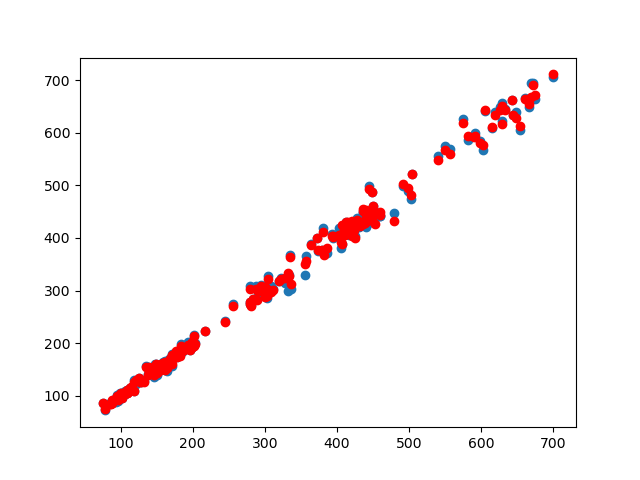
\includegraphics[scale = 0.9]{stock_prediction.png}
  \caption{Results of the linear regression neuron predicting the stock.}
\end{figure}

Something additional that could enhance the realism of our predictions is incorporating the concept of
prediction intervals. By considering the minimum and maximum discrepancies observed during training, we can
construct a range, denoted as $[min(\varepsilon_t), max(\varepsilon_t)]$, where $\varepsilon_t$ represents the
prediction error for a given observation. After making a prediction, we can introduce a random noise component
drawn from this range to add variability and make the predictions more realistic. It is crucial to pay
attention to this aspect if we aim to generate accurate and reliable predictions.

\section{The problems with a linear regression neuron}
 training prediction neurons poses a greater challenge compared
to classification neurons. The task of prediction involves an infinite approximation, striving to create a
model that can predict outcomes with minimal error, ideally achieving $\varepsilon = 0$. However, in
real-world
scenarios, perfect predictions are seldom attainable due to the inherent complexity and non-linearity of the
underlying problems. As we explored in the previous chapter, real-world data rarely exhibits a perfectly
straight pattern, making it more difficult to develop accurate prediction models. Consequently, we often
encounter the need to incorporate additional neurons and employ advanced techniques to effectively handle
these non-linear problems and achieve more realistic predictions. While delving into the depths of non-linear
problems is beyond the scope of this discussion, it is worth noting that the solution lies in utilizing more
neurons and constructing more complex structures to minimize the error term $\varepsilon \approx 0$. To echo the
sentiments expressed in the previous chapter, the necessity for more neurons and sophisticated architectures
becomes apparent. Thus, I won't delve deeper into this topic since it was thoroughly addressed
\hyperref[sec:problems-with-the-perceptron]{in the
previous chapter}.
